\section{无约束优化最优性问题}
\subsection{无约束优化最优性条件}

数学模型$\min\limits_{\boldsymbol{x}\in\mathbb{R}^n}f(\boldsymbol{x})$,其中$f:\mathbb{R}^n\to \mathbb{R}$

\begin{note}
    最优解判定:
    \begin{itemize}
        \item 直观地,验证最优解,需将其和附近点的目标函数值逐一比较,工作量太大。
        \item 利用目标函数的连续可微性质,可建立一个简易的判断方法, 这就是光滑优化问题的最优性条件.
    \end{itemize}
\end{note}

\begin{theorem}[无约束优化问题]
    $\boldsymbol{x}^*$是$\min\limits_{\boldsymbol{x}\in\mathbb{R}^n}f(\boldsymbol{x})$(局部)最优解,则$\nabla f(\boldsymbol{x}^*) = \boldsymbol{0}$
\end{theorem}
\begin{proof}
    反证法。取$\boldsymbol{d} = -\nabla f(\boldsymbol{x}^*)$,$\alpha>0$充分小。则
    \[
        \begin{array}{ll}
            f(\boldsymbol{x}^*+\alpha\boldsymbol{d})&=f(\boldsymbol{x}^*)+\alpha\nabla f(\boldsymbol{x}^*)^\mathrm{T}\boldsymbol{d}+o(\alpha)\\
            &=f(\boldsymbol{x}^*)-\alpha\|\nabla f(\boldsymbol{x}^*)\|^2+o(\alpha)\\
            &<f(\boldsymbol{x}^*)
        \end{array}
    \]
    和$\boldsymbol{x}^*$是$\min\limits_{\boldsymbol{x}\in\mathbb{R}^n}f(\boldsymbol{x})$(局部)最优解矛盾。证毕!
\end{proof}
\begin{definition}[凸函数]
    $f\left(\lambda\boldsymbol{x}+(1-\lambda)\boldsymbol{y}\right)\leqslant\lambda f(\boldsymbol{x})+(1-\lambda)f(\boldsymbol{y}),\forall\boldsymbol{x},\boldsymbol{y}\in\mathbb{R}^n,\lambda\in[0,1]$或者$f\left(\sum\limits_{i=1}^m\lambda_i\boldsymbol{x}_i\right)\leqslant\sum\limits_{i=1}^m\lambda_if(\boldsymbol{x}_i),\forall \boldsymbol{x}_i\in\mathbb{R}^n,\lambda_i\geqslant 0,i=1,2,\cdots,m,\sum\limits_{i=1}^m\lambda_i=1$
\end{definition}
\begin{definition}[凸组合]
    设$\boldsymbol{x}_1,\boldsymbol{x}_2,\cdots ,\boldsymbol{x}_m\in\mathbb{R}^n$,$\lambda_{1}+\lambda_{2}+\cdots+\lambda_{m}=1,\lambda_{1},\lambda_{2},\cdots,\lambda_{m}\in (0,1)$,则称$\lambda_1\boldsymbol{x}_1+\lambda_2\boldsymbol{x}_2+\cdots+\lambda_m\boldsymbol{x}_m$为$\boldsymbol{x}_1,\boldsymbol{x}_2,\cdots ,\boldsymbol{x}_m$的一个凸组合。
\end{definition}
\begin{definition}[凸函数的等价定义1(上图)]
    函数$f$的上图$\operatorname{epi}(f)$是凸集。$\operatorname{epi}(f):=\{(\boldsymbol{x},\alpha)\in\mathbb{R}^n\times\mathbb{R}\mid\alpha\geqslant f(\boldsymbol{x})\}$是凸集。
    \begin{figure}[H]
        \centering
        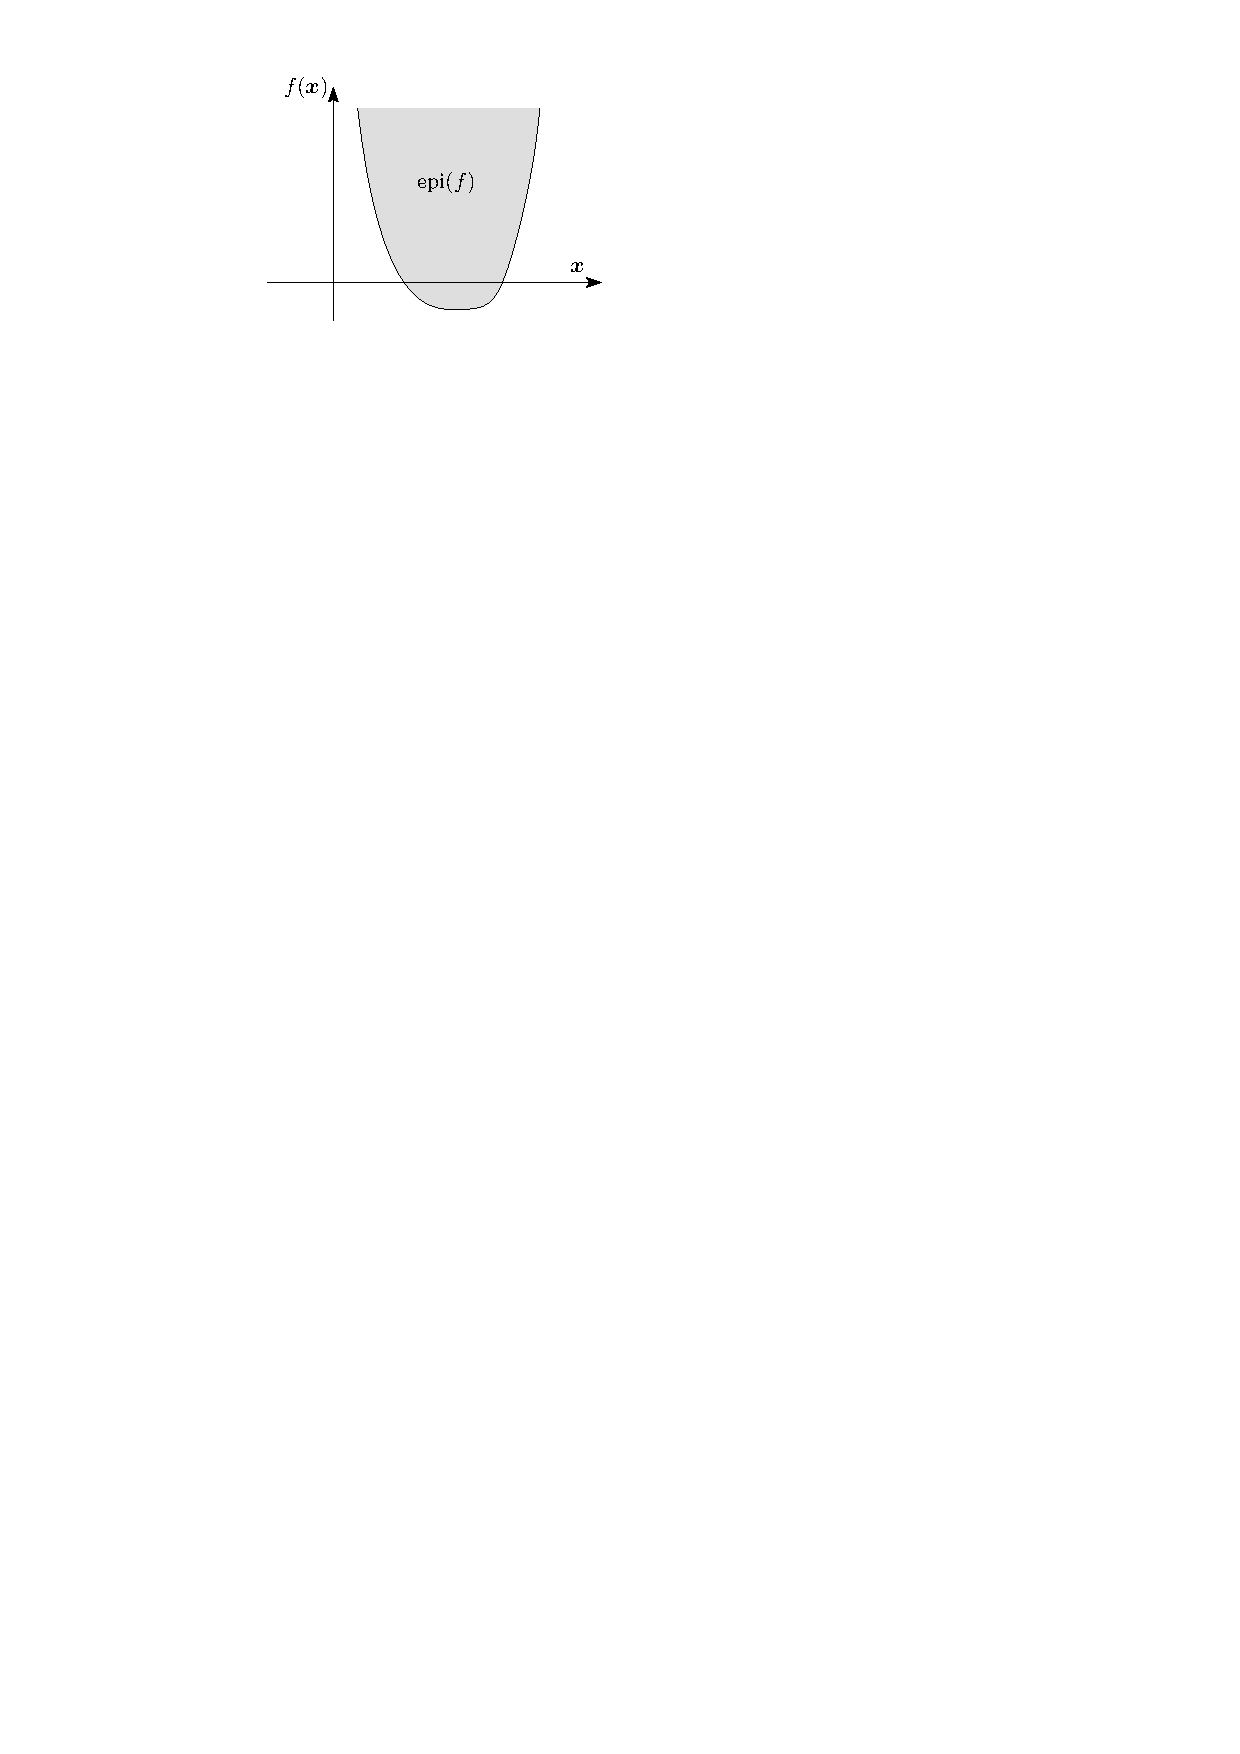
\includegraphics{image/epi.pdf}
    \end{figure}
\end{definition}
\begin{definition}[凸函数的等价定义2(连续可微)]
    切平面在曲面下方。
    $f(\boldsymbol{y})-f(\boldsymbol{x})\geqslant\nabla f(\boldsymbol{x})^{\mathrm{T}}(\boldsymbol{y}-\boldsymbol{x}),\forall \boldsymbol{x},\boldsymbol{y}\in\mathbb{R}^{n}$
\end{definition}
\begin{definition}[凸函数的等价定义3(二阶连续可微)]
    $\boldsymbol{h}^{T}\nabla f(\boldsymbol{x})\boldsymbol{h}\geqslant 0,\forall \boldsymbol{x},\boldsymbol{h}\in \mathbb{R}^n$
\end{definition}
\begin{definition}[一致凸函数(凸函数的加强版)]
    对函数$f:\mathbb{R}^n\to \mathbb{R}$,若存在$\eta>0$,使对任意$\boldsymbol{x},\boldsymbol{y}\in \mathbb{R}$和$\lambda\in (0,1)$成立
    \[
        f(\lambda\boldsymbol{x}+(1-\lambda)\boldsymbol{y})\leqslant\lambda f(\boldsymbol{x})+(1-\lambda)f(\boldsymbol{y})-\lambda(1-\lambda)\eta\|\boldsymbol{x}-\boldsymbol{y}\|^2
    \]
    则称其为一致凸函数,又称强凸函数。
    \begin{figure}[H]
        \centering
        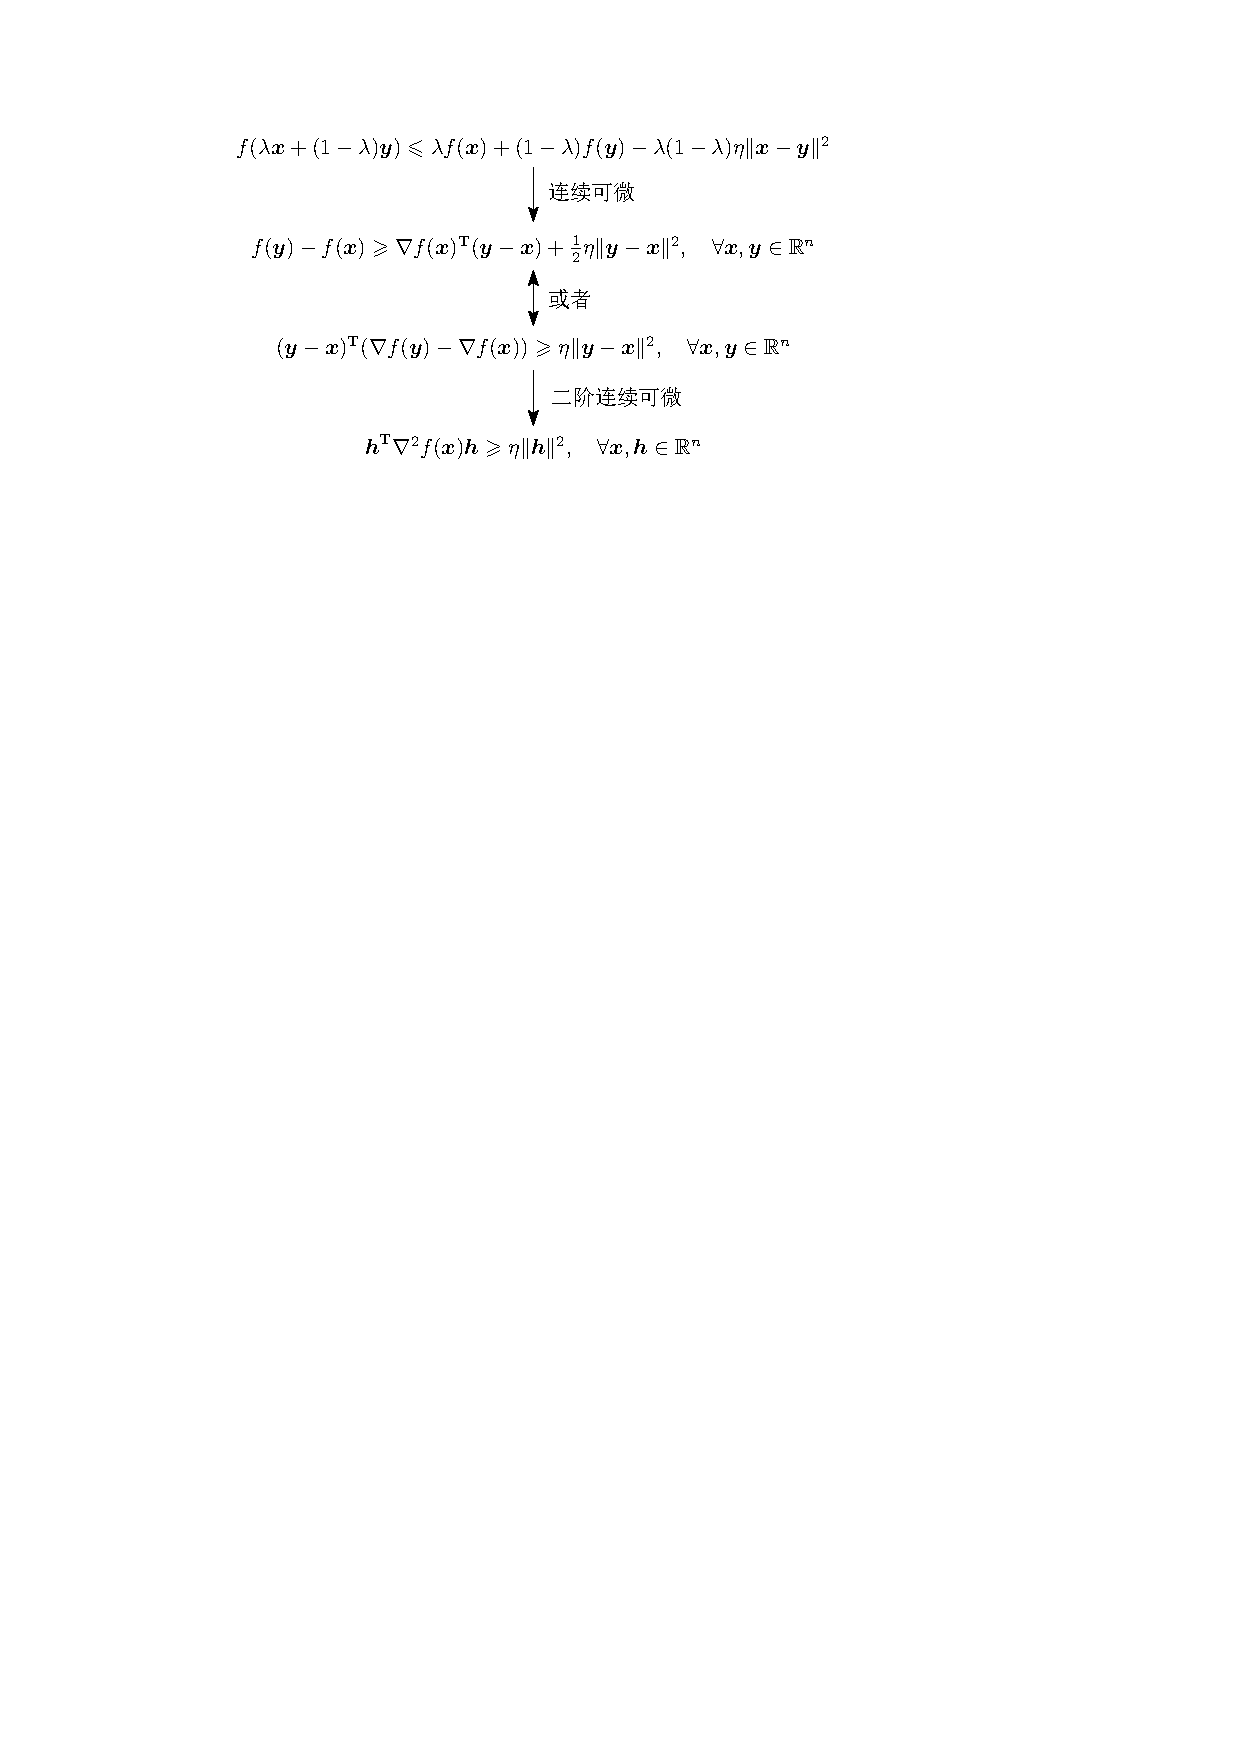
\includegraphics{image/一致凸函数.pdf}
    \end{figure}
\end{definition}
\begin{note}
    线性函数是凸函数但不一致凸。对二次函数,一致凸与严格凸等价。
\end{note}
\begin{note}
    $f(\boldsymbol{x})$一致凸等价于$f(\boldsymbol{x})-\eta \|\boldsymbol{x}\|^2$为凸函数,存在$\eta>0$
\end{note}
\begin{theorem}[凸优化]
    $\min\limits_{\boldsymbol{x}\in\mathbb{R}^n}f(\boldsymbol{x})$,$f:\mathbb{R}^n\to \mathbb{R}$为连续可微的凸函数。凸优化问题的稳定点为其全局最优解。
\end{theorem}
\begin{proof}
    利用凸函数的性质
    \[
        \begin{array}{c}
            f(\boldsymbol{x})-f(\boldsymbol{x}^*)\geqslant \left<\nabla f(\boldsymbol{x}^*),\boldsymbol{x}-\boldsymbol{x}^*\right> = 0\\
            f(\boldsymbol{x})>f(\boldsymbol{x}^*)
        \end{array}
    \]
\end{proof}
\begin{theorem}[无约束优化二阶最优性条件]
    设$\boldsymbol{x}^*$为优化问题$\min\limits_{\boldsymbol{x}\in\
    \mathbb{R}^n}f(\boldsymbol{x})$的最优解,则$\nabla f(\boldsymbol{x}^*) = \boldsymbol{0},\nabla^2f(\boldsymbol{x}^*)$半正定。
\end{theorem}
\begin{proof}
    结论$\nabla f(\boldsymbol{x}^{*})=\mathbf{0}$已证。
    
    反设$\nabla^2 f(\boldsymbol{x}^{*})$非半正定,则存在向量$\boldsymbol{d}$使得
    \[
        \boldsymbol{d}^\mathrm{T}\nabla^2f(\boldsymbol{x^*})\boldsymbol{d}<0.
    \]
    取$\alpha>0$充分小。由泰勒展开式
    \[
        \begin{array}{ll}
            f(\boldsymbol{x}^{*}+\alpha\boldsymbol{d})& =f(\boldsymbol{x}^{*})+\alpha\nabla f(\boldsymbol{x}^{*})^{\mathrm{T}}\boldsymbol{d}+\frac{1}{2}\alpha^{2}\boldsymbol{d}^{\mathrm{T}}\nabla^{2}f(\boldsymbol{x}^{*})\boldsymbol{d}+o(\alpha^{2})  \\
            &<f(\boldsymbol{x}^{*}).
        \end{array}
    \]
    得矛盾。证毕!
\end{proof}
\begin{note}
    二阶必要条件的非充分性:
    
    函数$f(x)$在零点满足$\nabla f(\boldsymbol{x}^*) = \boldsymbol{0}$,$\nabla^2f(\boldsymbol{x})$半正定,但但零点不是其最优值点。
\end{note}
\begin{theorem}[二阶充分条件]
    对优化问题$\min\limits_{\boldsymbol{x}\in \mathbb{R}^n}f(\boldsymbol{x})$,设$\nabla f(\boldsymbol{x}) = \boldsymbol{0}$,$\nabla^2\boldsymbol{f(\boldsymbol{x}^*)}$正定,则$\boldsymbol{x}^*$为该优化问题的严格最优解
\end{theorem}
\begin{proof}
    对任意充分靠近$\boldsymbol{x}^*$的$\boldsymbol{x}$,存在单位向量$\boldsymbol{d}$,使得
    \[
        \boldsymbol{x} = \boldsymbol{x}^*+\alpha\boldsymbol{d}   
    \]
    其中$\alpha>0$充分小。则
    \[
        f(\boldsymbol{x})=f(\boldsymbol{x}^{*})+\frac{1}{2}\alpha^{2}\boldsymbol{d}^{\mathrm{T}}\nabla^{2}f(\boldsymbol{x}^{*})\boldsymbol{d}+o(\alpha^{2})>f(\boldsymbol{x}^{*}).
    \]
\end{proof}
\begin{example}
    $\min\limits_{x>0,y\geqslant 0}f(x,y)=\dfrac{10}{x}+\dfrac{(x-y)^{2}}{2x}+\dfrac{3y^{2}}{2x}$\quad \Stars{5}

    先忽略约束:利用$\min\limits_{x,y}f(x,y)=\min\limits_x\min\limits_yf(x,y)$,先固定$x$,关于$y$做内层优化,再求解关于$x$的外层优化
    \[
        \min\limits_{y}f(x,y)=\frac{10}{x}+\frac{(x-y)^{2}}{2x}+\frac{3y^{2}}{2x}
    \]
    目标函数关于$y$为凸函数,利用最优性条件得最优解
    \[
        \begin{array}{c}
            f(x,y)=\dfrac{1}{2x}\left( 20+x^2-2xy+4y^2 \right)\\
            y = \dfrac{1}{4}x
        \end{array}
    \]
    将上述最优解代入目标函数得外层优化问题
    \[
        \min f(x)=\dfrac{10}{x}+\dfrac{3}{8}x
    \]
    目标函数关于$x$为凸函数(二阶导数大于0)。再利用最优性条件得$x=\frac43\sqrt{15},y=\frac{1}{4}x=\frac{1}{3}\sqrt{15}$

    它们满足约束条件,自然为原问题的最优解。
\end{example}

\subsection{无约束优化线搜索方法}
\subsubsection{精确线搜索方法}
\begin{note}
    优化模型:
    \[
        \min\limits_{\boldsymbol{x}\in\mathbb{R}^n}f(\boldsymbol{x})
    \]
    其中,$f:\mathbb{R}^n\to\mathbb{R}$连续可微。
\end{note}
\begin{note}
    有关记号:
    \[
        \begin{array}{ll}
            \boldsymbol{g}_k=\nabla f(\boldsymbol{x}_k), & \boldsymbol{g}(\boldsymbol{x})=\nabla f(\boldsymbol{x})\\
            \boldsymbol{G}_k=\nabla^2f(\boldsymbol{x}_k), & \boldsymbol{G}(\boldsymbol{x})=\nabla^2f(\boldsymbol{x}).
        \end{array}
    \]
\end{note}
我们先回顾作为最速下降方向的负梯度方向。假设$\nabla f(\boldsymbol{x})\neq \boldsymbol{0}$。固定方向$\boldsymbol{d}\in \mathbb{R}^n$且$\|\boldsymbol{d}\| = 1$。考虑沿此方向函数值的变化。由可微的定义可知
\[
    f(\boldsymbol{x}+\tau \boldsymbol{d}) = f(\boldsymbol{x}) + \tau \nabla f(\boldsymbol{x})^{\mathrm{T}}\boldsymbol{d} + o(\tau),\ \tau>0
\]
当$\nabla f(\boldsymbol{x})^{\mathrm{T}}\boldsymbol{d}<0 $时,由于$\frac{o(\tau)}{\tau}\to 0,\tau\to 0_{+}$可知,存在$\varepsilon >0$,使得当$0<\tau<\varepsilon$时,
\[
    \dfrac{o(\tau)}{\tau}\leq -\dfrac{\nabla f(\boldsymbol{x})^{\mathrm{T}}\boldsymbol{d}}{2}
\]
此时
\[
    f(\boldsymbol{x}+\tau \boldsymbol{d})-f(\boldsymbol{x})\leq \dfrac{\tau}{2}\cdot \nabla f(\boldsymbol{x})^{\mathrm{T}}\boldsymbol{d}< 0
\]
上式表明,从$\boldsymbol{x}$点沿$\boldsymbol{d}$方向出发,当步长$\tau <\varepsilon$时,
\[
    f(\boldsymbol{x}+\tau \boldsymbol{d})<f(\boldsymbol{x})
\]
因此,称满足条件$\nabla f(\boldsymbol{x})^{\mathrm{T}}\boldsymbol{d}<0$的方向为下降方向。而称下降最快或$\nabla f(\boldsymbol{x})^{\mathrm{T}}\boldsymbol{d}$最小的方向为最速下降方向,也即
\[
    \begin{array}{c}
        \hat{\boldsymbol{d}} = \arg\min \{\nabla f(\boldsymbol{x})^{\mathrm{T}}\boldsymbol{d}\}\\
        \text{s.t.} \|\boldsymbol{d}\|=1
    \end{array} 
\]
则$\boldsymbol{d} = -\frac{\nabla f(\boldsymbol{x})}{\|\nabla f(\boldsymbol{x})\|}$。事实上,有Cauchy-Schwarz不等式
\[
    |\nabla f(\boldsymbol{x})^{\mathrm{T}} \boldsymbol{d}|\leq \|\nabla f(\boldsymbol{x}) \|\cdot \|\boldsymbol{d} \|\leq \|\nabla f(\boldsymbol{x}) \|
\]
可知
\[
    -\|\nabla f(\boldsymbol{x}) \| \leq \nabla f(\boldsymbol{x})^{\mathrm{T}} \boldsymbol{d} \leq \|\nabla f(\boldsymbol{x}) \|
\]
从而$\hat{\boldsymbol{d}} = \dfrac{\nabla f(\boldsymbol{x})}{\|\nabla f(\boldsymbol{x})\|}$可取得下界$-\|\nabla f(\boldsymbol{x}) \|$。
\begin{note}
    算法分析:
    \begin{itemize}
        \item 迭代过程:$\boldsymbol{x}_{k+1} = \boldsymbol{x}_k+\alpha_k \boldsymbol{d}_k$
        \item 精确线搜索(最优步长):$\alpha = \arg\min\limits_{\alpha\geqslant 0}f(\boldsymbol{x}_k+\alpha\boldsymbol{d}_k)$
        \item $\left\{ \boldsymbol{x}_{n} \right\}$满足$\left\{ f(\boldsymbol{x}) \right\}$递减,$\nabla f(\boldsymbol{x})\to 0$
        \item 沿下降方向寻求目标函数的最大下降点
        \item 基本性质:$f(\boldsymbol{x}_{k}+\alpha_{k}\boldsymbol{d}_{k})\leqslant f(\boldsymbol{x}_{k}+\alpha \boldsymbol{d}_{k}),\quad\forall\alpha>0$
        \[
            f_{\alpha}^{\prime}(\boldsymbol{x}_{k}+\alpha_{k}\boldsymbol{d}_{k})=\nabla f(\boldsymbol{x}_{k}+\alpha_{k}\boldsymbol{d}_{k})^{\mathrm{T}}\boldsymbol{d}_{k}=0
        \]
    \end{itemize}
\end{note}

\begin{itemize}
    \item 最优步长的计算:一元函数的极值问题,全局最优步长难求.通常只能求得局部最优或近似最优步长。
    \item 常用的方法:黄金分割法、多项式插值
\end{itemize}

精确线搜索下降算法:
\begin{enumerate}
    \item 取初始点$\boldsymbol{x}_0\in\mathbb{R}^n$和参数$\varepsilon\geqslant 0$,令$k = 0$
    \item 若$\|\boldsymbol{g}_k\|\leqslant \varepsilon$,算法终止;否则进入下一步
    \item 计算下降方向$\boldsymbol{d}_k$满足$\boldsymbol{g}_k^{\mathrm{T}}\boldsymbol{d}_k<0$
    \item 计算步长
    \[
        \alpha_{k}=\arg\min\{f(\boldsymbol{x}_{k}+\alpha\boldsymbol{d}_{k})\mid\alpha\geqslant 0\}
    \]
    \item 令$\boldsymbol{x}_{k+1}=\boldsymbol{x}_{k}+\alpha_{k}\boldsymbol{d}_{k},\,k=k+1$,转步2
\end{enumerate}

\begin{note}
    算法收敛性:要保证算法收敛,要对搜索方向、目标函数做些假设。
    \begin{theorem}
        设目标函数$f\in C^2\text{(二阶连续)}$有下界
        
        下降方向$\boldsymbol{d}_k$与负梯度方向$-\boldsymbol{g}_k$夹角满足
        \[
            \theta_k\leqslant\dfrac{\pi}{2}-\theta,0<\theta\leqslant\dfrac{\pi}{2}   
        \]

        若精确线搜索方法产生无穷迭代点列,且满足
        $\| \nabla^2 f(\boldsymbol{x}_k+\alpha\boldsymbol{d}_k) \|\leqslant M,\,\forall \alpha>0$,\newline
        其中,$M>0$为常数,则算法收敛,即$\lim\limits_{k\to \infty}\boldsymbol{g}_k = \boldsymbol{0}$
    \end{theorem}
\end{note}

\subsubsection{非精确线搜索方法}
\begin{note}
    最优步长的缺陷:
    \begin{itemize}
        \item 最优步长的初衷是在每一迭代步使目标函数下降量达到最大.但计算量太大,而且不好求. 
        \item 最优化问题关注全局最优值点。集中于某个方向上的线搜索似乎没有必要。
    \end{itemize}
\end{note}

设$\boldsymbol{d}_k$为$\boldsymbol{x}_k$的下降方向,即$\boldsymbol{d}_{k}^{\mathrm{T}}\boldsymbol{g}_k<0$,对$\sigma\in\left( 0,1 \right)$,只要$\alpha>0$充分小,有
\[
    f(\boldsymbol{x}_k+\alpha\boldsymbol{d}_k) = f(\boldsymbol{x}_k)+\alpha \boldsymbol{g}_{k}\boldsymbol{d}_k+o(\alpha)<0
\]

步长选取:先取一个较大的步长, 看目标函数是否有满意的下降量。否则依次按比例压缩,直至满足要求。又称进退试探法。
\begin{definition}[Armijo步长规则]
    取常数$\beta>0,\sigma,\gamma\in(0,1)$。步长$\alpha_k = \beta \gamma^{m_k}$,其中$m_k$为$0,1,\cdots$中满足下式的最小值
    \[
        f(\boldsymbol{x}_k+\beta\gamma^m\boldsymbol{d}_k) \leqslant f_k+\sigma\beta\gamma^m\boldsymbol{g}_k^{\mathrm{T}}\boldsymbol{d}_k
    \]

    如$\alpha_k<\beta$,则
    \[
        \begin{array}{c}
            f(\boldsymbol{x}_k+\beta\gamma^{\colorbox{red!30}{$m_k$}}\boldsymbol{d}_k)\leqslant f(\boldsymbol{x}_k)+\sigma\beta\gamma^{m_k}\boldsymbol{g}_k^{\mathrm{T}}\boldsymbol{d}_k\\
            f(\boldsymbol{x}_k+\beta\gamma^{\colorbox{red!30}{$m_k-1$}}\boldsymbol{d}_k)> f(\boldsymbol{x}_k)+\sigma\beta\gamma^{m_k-1}\boldsymbol{g}_k^{\mathrm{T}}\boldsymbol{d}_k
        \end{array}
    \]
\end{definition}

\begin{definition}[Wolfe步长]
    常数$0<\sigma_{1}<\sigma_{2}<1$。步长$\alpha_k$同时满足
    \[
        f(\boldsymbol{x}_{k}+\alpha\boldsymbol{d}_{k})\leqslant f(\boldsymbol{x}_{k})+\sigma_{1}\alpha\boldsymbol{g}_{k}^{\mathrm{T}}\boldsymbol{d}_{k}\quad \colorbox{cyan!50}{下降性条件}
    \]
    和
    \[
        \nabla f(\boldsymbol{x}_{k}+\alpha\boldsymbol{d}_{k})^{\mathrm{T}}\boldsymbol{d}_{k}\geqslant\sigma_{2}\boldsymbol{g}_{k}^{\mathrm{T}}\boldsymbol{d}_{k} \Longleftrightarrow \boldsymbol{g}_{k+1}^{\mathrm{T}}\boldsymbol{d}_{k}\geqslant\sigma_{2}\boldsymbol{g}_{k}^{\mathrm{T}}\boldsymbol{d}_{k}\\
    \]
    曲线\colorbox{cyan!50}{$\varphi_{k}(\alpha)=f(\boldsymbol{x}_{k}+\alpha\boldsymbol{d}_{k})$}的陡度\colorbox{cyan!50}{$\nabla f(\boldsymbol{x}_{k}+\alpha\boldsymbol{d}_{k})^{\mathrm{T}}\boldsymbol{d}_{k}$}比$\alpha = 0$点有所减缓从而远离当前迭代点
\end{definition}
\begin{figure}[H]
    \centering
    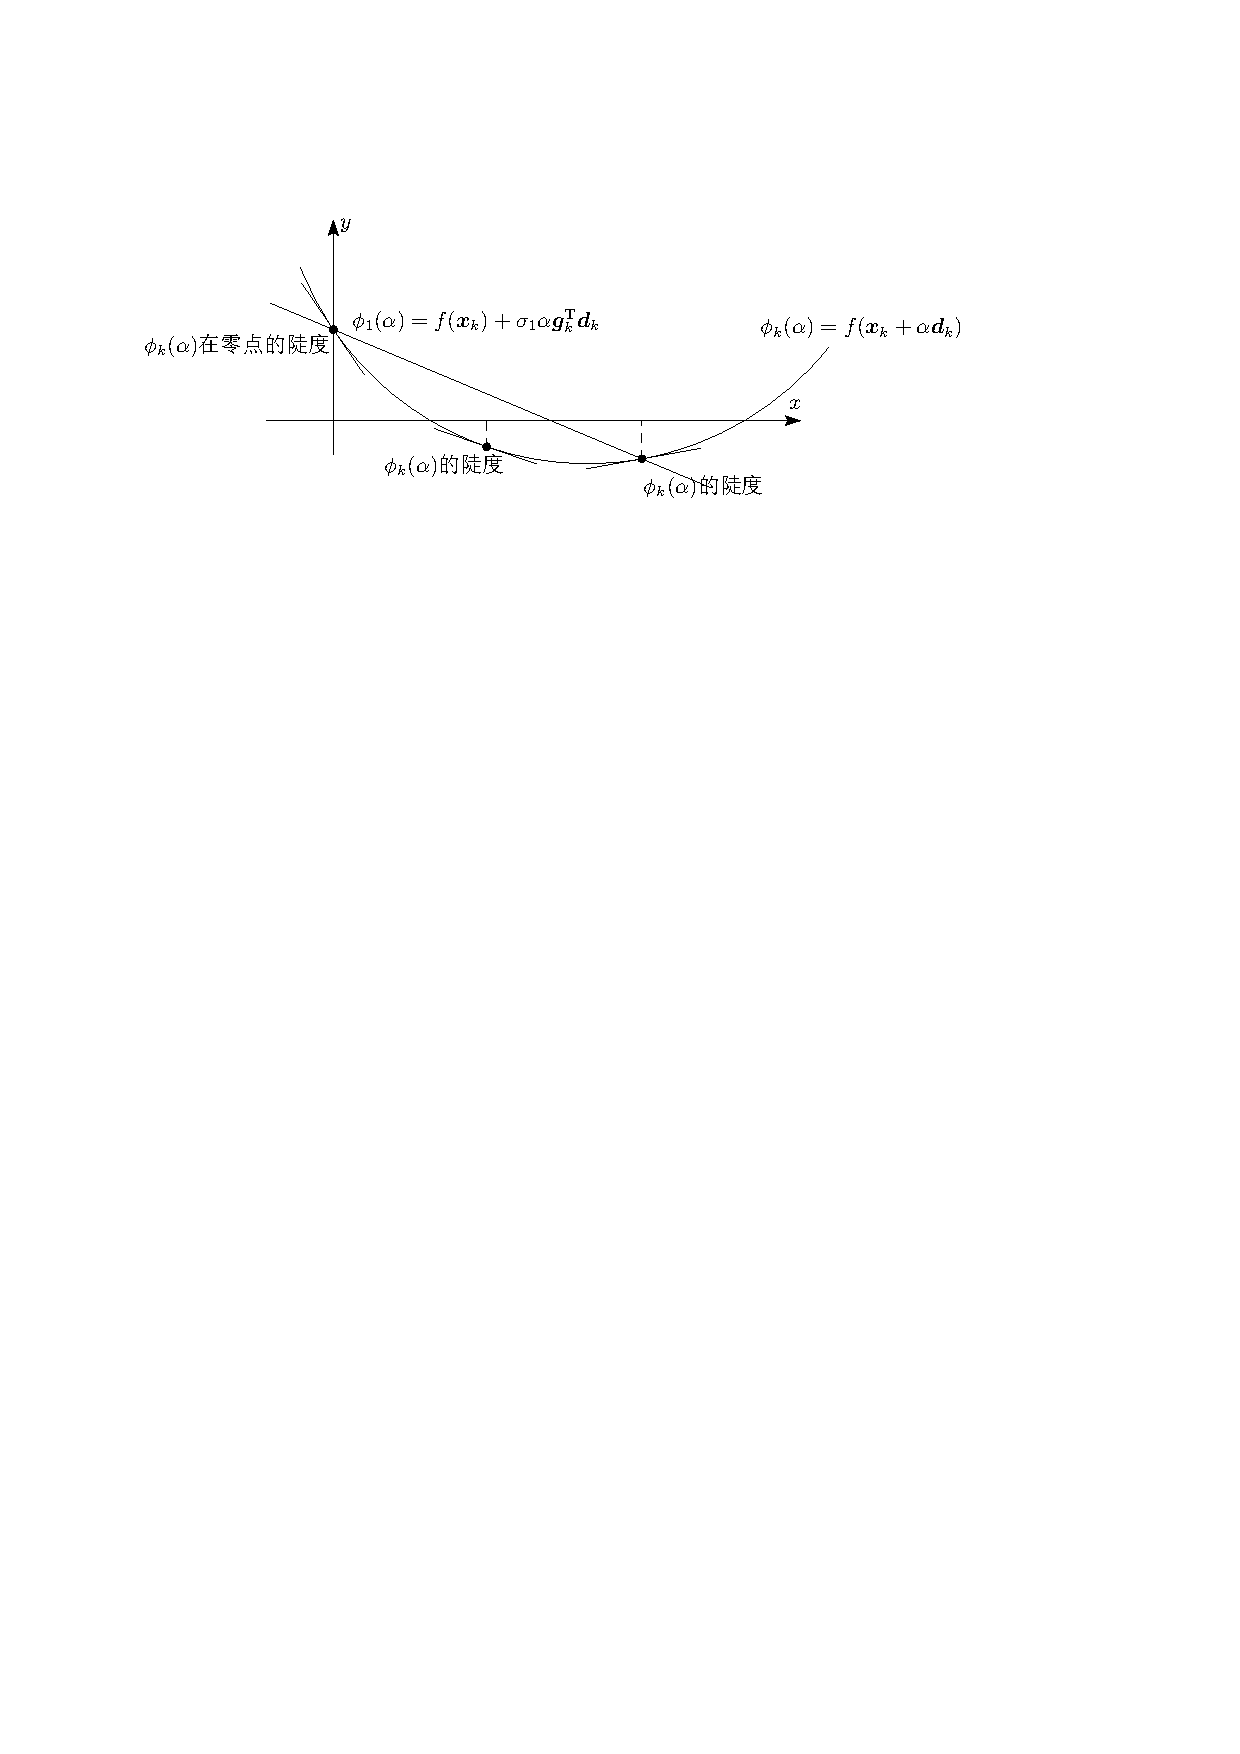
\includegraphics[]{image/Wolfe步长.pdf}
\end{figure}
\subsection{最速算法与牛顿算法}

\subsubsection{最速下降算法}
优化模型$\min\limits_{\boldsymbol{x}\in\mathbb{R}^n}f(\boldsymbol{x})$

迭代算法
\[
    \begin{array}{c}
        \boldsymbol{x}_{k+1} = \boldsymbol{x}_{k} + \alpha_{k}\boldsymbol{d}_{k} \\
        \alpha_{k} = \arg\min\limits_{\alpha\in \mathbb{R}_{+}}f(\boldsymbol{x}_k+\alpha\boldsymbol{d}_k)\\
        \boldsymbol{d}_{k} = -\nabla f(\boldsymbol{x}_k)
    \end{array}  
\]
\begin{corollary}[最优步长规则下的收敛性质]
    最优步长规则下的收敛性质$\boldsymbol{d}_{k}^{\mathrm{T}}\boldsymbol{d}_{k+1} = 0$
\end{corollary}
\begin{proof}
    记$\varphi_k(\alpha)=f(\boldsymbol{x}_k+\alpha\boldsymbol{d}_k).$,利用最优步长规则
    \[
        \begin{aligned}
            0 & =\varphi_{k}^{\prime}(\alpha_{k})=\langle\nabla f(x_{k}+\alpha_{k}\boldsymbol{d}_{k}),\boldsymbol{d}_{k}\rangle   \\
            &=\langle\nabla f(\boldsymbol{x}_{k+1}),\boldsymbol{d}_k\rangle  \\
            &=-\langle\boldsymbol{d}_{k+1},\boldsymbol{d}_{k}\rangle.
        \end{aligned}
    \]
\end{proof}
\begin{theorem}[收敛速度估计]
    对严格凸二次函数$f(\boldsymbol{x}) = \dfrac{1}{2}\boldsymbol{xG}{\mathrm{T}}\boldsymbol{x}$,$\lambda_1\geqslant\lambda_2\geqslant\cdots\geqslant \lambda_n>0$为矩阵$\boldsymbol{G}$的特征根。则最优步长最速下降算法线性收敛,即
    \[
        \frac{f_{k+1}-f(\boldsymbol{x}^*)}{f_k-f(\boldsymbol{x}^*)}\leqslant\Big(\frac{\lambda_1-\lambda_n}{\lambda_1+\lambda_n}\Big)^2,\quad \frac{\lVert\boldsymbol{x}_{k+1}-\boldsymbol{x}^*\rVert}{\lVert\boldsymbol{x}_k-\boldsymbol{x}^*\rVert}\leqslant\frac{\lambda_1-\lambda_n}{\lambda_1+\lambda_n}\sqrt{\frac{\lambda_1}{\lambda_n}}.
    \]
    \begin{itemize}
        \item  很强条件下(二次严格凸)最速下降算法的收敛速度估计;
        \item  线性收敛是一个很慢的收敛速度;
        \item 有例为证:该理论估计是准确的,没有提升的空间。
    \end{itemize}
\end{theorem}
\begin{example}
    $\min\limits_{\boldsymbol{x}\in\mathbb{R}^2}f(x_1,x_2) = \dfrac{1}{3}x_{1}^2+\dfrac{1}{2}x_2^2$。\Stars{5}
    
    显然,唯一最优解$\boldsymbol{x}^* = \left( 0,0 \right)$,取初始点$\boldsymbol{x}_0 = (3,2)$,那么最速下降方法产生的迭代点列
    $\boldsymbol{d}_0$
    \[
        \boldsymbol{x}_{k}=\left(\frac{3}{5^{k}};(-1)^{k}\frac{2}{5^{k}}\right)\overset{k\to\infty}{\longrightarrow}(0;0)
    \]
    全局收敛,收敛速度线性!
    有$\|\boldsymbol{x}_k-\boldsymbol{x}^*\|=\sqrt{13}\big(\frac15\big)^k.$那么
    \[
        \begin{aligned}
            \frac{\|\boldsymbol{x}_{k+1}-\boldsymbol{x}^*\|}{\|\boldsymbol{x}_k-\boldsymbol{x}^*\|} & =\frac15<\frac15\sqrt{\frac32}=\frac{\lambda_1-\lambda_2}{\lambda_1+\lambda_2}\sqrt{\frac{\lambda_1}{\lambda_2}}\\
            \frac{f(\boldsymbol{x}_{k+1})-f(\boldsymbol{x}^*)}{f(\boldsymbol{x}_k)-f(\boldsymbol{x}^*)} & =\frac1{25}=\left(\frac{\lambda_1-\lambda_2}{\lambda_1+\lambda_2}\right)^2
        \end{aligned}
    \]
\end{example}
\begin{note}
    优点:
    \begin{itemize}
        \item 迭代过程简单,计算量与存储量小;
        \item 初始步函数值下降较快,可以快速靠近最优解。
    \end{itemize}

    缺点:
    \begin{itemize}
        \item 相邻两搜索方向正交,导致锯齿现象:越靠近最优值点,靠近速度越慢。
        \item 不适于算法收局。
    \end{itemize}
\end{note}

\subsubsection{牛顿算法}
\[
    \min\limits_{\boldsymbol{x}\in\mathbb{R}^n}f(\boldsymbol{x})
\]
利用目标函数$f(\boldsymbol{x}_k+\boldsymbol{d})$在$\boldsymbol{x}_k$的二阶近似求新的迭代点
\[
    m_k(\boldsymbol{d})\triangleq f(\boldsymbol{x}_k)+\boldsymbol{d}^\mathrm{T}\boldsymbol{g}_k+\frac{1}{2}\boldsymbol{d}^\mathrm{T}\boldsymbol{G}_k\boldsymbol{d}.
\]
利用最优性条件
\[
    \nabla_{\boldsymbol{d}} m_{k}(\boldsymbol{d}) = \boldsymbol{g}_{k}+\boldsymbol{G}_{k}\boldsymbol{d} = \boldsymbol{0} \longrightarrow \boldsymbol{d}_{k}^{N} = -\boldsymbol{G}_{k}^{-1}\boldsymbol{g}_{k}  
\]
令$\boldsymbol{x}_{k+1} = \boldsymbol{x}_{k}-\boldsymbol{G}_{k}^{-1}\boldsymbol{g}_{k}$,即得牛顿算法。牛顿步
\[
    \boldsymbol{d}_{k}^{N} = -\boldsymbol{G}_{k}^{-1}\boldsymbol{g}_{k}
\]
\begin{theorem}
    设目标函数二阶连续可微,Hesse阵在最优值点$\boldsymbol{x}^*$非奇异.则
    \begin{enumerate}
        \item 若初始点充分靠近最优值点,则算法超线性收敛,$\lim\limits_{k\to\infty}\boldsymbol{x}_{k} = \boldsymbol{x}^*$                          
        \item 若Hesse阵在最优值点附近Lipschitz连续, 则二阶收敛。
    \end{enumerate}
\end{theorem}
\begin{proof}
    利用目标函数二阶展式
    \[
        \mathbf{0}=\boldsymbol{g}(x^*)=\boldsymbol{g}_k+\boldsymbol{G}_k(x^*-\boldsymbol{x}_k)+o(\|\boldsymbol{x}_k-\boldsymbol{x}^*\|).
    \]
    左乘$\boldsymbol{G}_{k}^{-1}$
    \[
        \begin{array}{l}
            \boldsymbol{x}_k-\boldsymbol{x}^*-\boldsymbol{G}_k^{-1}\boldsymbol{g}_k=o(\|\boldsymbol{x}_k-\boldsymbol{x}^*\|)\\
            \Rightarrow \boldsymbol{x}_{k+1}-\boldsymbol{x}^{*}=o(\|\boldsymbol{x}_{k}-\boldsymbol{x}^{*}\|). 
        \end{array}
    \]
    证毕!
\end{proof}
\begin{note}
    算法特点:
    \begin{itemize}
        \item 无全局收敛性。仅局部收敛,即要求初始点靠近最优值点;
        \item 二阶收敛:迭代点越靠近最优值点, 收敛速度越快!
        \item 具有二次终止性:对严格凸二次函数,一步即得最优解
        \item 严格二次函数$f(\boldsymbol{x})=\frac12\boldsymbol{x}^{\mathrm{T}}\boldsymbol{G}\boldsymbol{x}+\boldsymbol{g}^{\mathrm{T}}\boldsymbol{x}+c\Rightarrow \boldsymbol{x}^* = -\boldsymbol{G}^{-1}\boldsymbol{g}$
        
        任意初始点$\boldsymbol{x}_{0}\in\mathbb{R}^n$
        \[
            \begin{aligned}
                \boldsymbol{x}_{1}& =\boldsymbol{x}_{0}-G^{-1}\nabla f(\boldsymbol{x}_{0})  \\
                &=\boldsymbol{x}_{0}-\boldsymbol{G}^{-1}(\boldsymbol{G}\boldsymbol{x}_{0}+\boldsymbol{g}) \\
                &=-\boldsymbol{G}^{-1}\boldsymbol{g}=\boldsymbol{x}^{*}.
            \end{aligned}
        \]
    \end{itemize}
\end{note}
\begin{example}
    用牛顿法求解$\min f(x)=\sqrt{1+x^2}$\quad\Stars{5}
    
    $0$为最优解
    
    目标函数导数$f'(x)=\dfrac{x}{\sqrt{1+x^2}}\quad f''(x)=\dfrac{1}{(1+x^2)^{3/2}}$
    
    迭代过程
    \[
        \begin{aligned}
            x_{k+1}& =x_{k}-\frac{f'(x_{k})}{f''(x_{k})}  \\
            &=x_{k}-x_{k}(1+x_{k}^{2}) \\
            &=-x_{k}^{3}
        \end{aligned}
    \]
    \begin{itemize}
        \item 当$x_0<1$,算法快速收敛到最优解;
        \item 当$x_0\geqslant 1$,算法不收敛
    \end{itemize}
\end{example}
% \begin{example}
%     用牛顿算法求解$\operatorname*{min}f(\boldsymbol{x})=4x_{1}^{2}+x_{2}^{2}-x_{1}^{2}x_{2}$

%     目标函数梯度信息
%     \[
%         \nabla f(\boldsymbol{x})=\begin{pmatrix}8x_1-2x_1x_2\\2x_2-x_1^2\end{pmatrix}\quad\nabla^2f(\boldsymbol{x})=\begin{pmatrix}8-2x_2&-2x_1\\-2x_1&2\end{pmatrix}
%     \]
% \end{example}
\begin{note}
    牛顿方法的缺陷
    \begin{itemize}
        \item 初始点远离最优解时,算法可能不收敛;
        \item Hesse矩阵奇异时,算法不可行;
        \item  计算量和存储量大:需计算目标函数的梯度和Hesse阵
    \end{itemize}
\end{note}

\subsection{共轭梯度法}
线性方程组($\boldsymbol{A}$对称正定):
\[
    \boldsymbol{Ax} = \boldsymbol{b}
\]
\begin{itemize}
    \item 经典算法:Gauss消元法、系数矩阵三角分解法
    \item 算法缺陷:计算时间随问题规模急速增长。
\end{itemize}

将问题转化为
\[
    \min f(\boldsymbol{x}) = \dfrac{1}{2}\boldsymbol{x}^{\mathrm{T}}\boldsymbol{Ax}-\boldsymbol{b}^{\mathrm{T}}\boldsymbol{x}
\]

\subsubsection{线性共轭方向法}

\begin{definition}[共轭方向]
    对对称正定阵$\boldsymbol{A}$,若$\boldsymbol{d}_1,\boldsymbol{d}_2\in\mathbb{R}^n$,满足$\boldsymbol{d}_{1}^{\mathrm{T}}\boldsymbol{Ad}_2 = 0$,则称$\boldsymbol{d}_1,\boldsymbol{d}_2$关于矩阵$\boldsymbol{A}$共轭,并称其为$A$的共轭方向。

    \textcolor{red}{共轭是正交的推广。}
\end{definition}

\begin{definition}[线性共轭方向的推广]
    若向量组$\boldsymbol{d}_1,\boldsymbol{d}_2,\cdots,\boldsymbol{d}_n$关于对称正定阵$\boldsymbol{A}$两两共轭,即满足
    \[
        \boldsymbol{d}_i\boldsymbol{A}\boldsymbol{d}_j  = 0,\,1\leqslant i\neq j\leqslant k
    \]
\end{definition}
\begin{corollary}
    若向量组$\boldsymbol{d}_1,\boldsymbol{d}_2,\cdots,\boldsymbol{d}_n$,关于矩阵$\boldsymbol{A}$共轭,则它们线性无关。
\end{corollary}

\begin{note}
    线性共轭方向法:
    \[
    \min\limits_{\boldsymbol{x}\in\mathrm{R}^n} f(\boldsymbol{x}) = \dfrac{1}{2}\boldsymbol{x}^{\mathrm{T}}\boldsymbol{Ax}-\boldsymbol{b}^{\mathrm{T}}x
    \]
    \begin{enumerate}
        \item 初始点$\boldsymbol{x}_0$,搜索方向$\boldsymbol{d}_0$满足$\left< \boldsymbol{d}_0,\boldsymbol{g}_0 \right><0$,终止参数$\varepsilon\geqslant 0$,令$k=0$
        \item 若$\|\boldsymbol{g}_k\|\leqslant \varepsilon$,算法终止;否则,进入下一步
        \item 计算最优步长$\alpha = \arg\min\limits_{\alpha\geqslant 0}\left\{ f(\boldsymbol{x}_k+\alpha \boldsymbol{d}_{k}) \right\}$,令$\boldsymbol{x}_{k+1} = \boldsymbol{x}_k+\alpha_k\boldsymbol{d}_k$
        \item 构造$\boldsymbol{d}_{k+1}$使其与$\boldsymbol{d}_0,\cdots,\boldsymbol{d}_k$关于矩阵$\boldsymbol{A}$共轭,令$k \gets k+1$,返回步2
    \end{enumerate}
\end{note}

\begin{theorem}[二次终止性]
    对严格凸二次函数$\min f(\boldsymbol{x}) = \dfrac{1}{2}\boldsymbol{x}^{\mathrm{T}}\boldsymbol{Ax}-\boldsymbol{b}^{\mathrm{T}}\boldsymbol{x}$,向量组$\boldsymbol{d}_0,\boldsymbol{d}_1,\cdots,\boldsymbol{d}_{n-1}$关于$\boldsymbol{A}$共轭。共轭方向发产生点列$\left\{ \boldsymbol{x}_{k} \right\}$。则对任意$0\leqslant k\leqslant n-1$,$\boldsymbol{x}_{k+1}$是目标函数在仿射集$\boldsymbol{x}_0+\operatorname{span}\left[ \boldsymbol{d}_0,\cdots,\boldsymbol{d}_{k} \right]$上的最小值点,算法至多$n$步迭代后终止。
\end{theorem}
\begin{example}
    利用共轭梯度法求$\boldsymbol{Ax} = \boldsymbol{b}$或者说,利用共轭梯度法求$\min x_1^2+\dfrac{1}{2}x_2^2+\dfrac{1}{2}x_3^2$\quad\Stars{5}


    其中,
    \[
        \boldsymbol{A} = \begin{bmatrix}
            1 & 0 & 0\\
            0 & \frac{1}{2} & 0 \\
            0 & 0 & \frac{1}{2}
        \end{bmatrix},\quad
        \boldsymbol{b} = \begin{pmatrix}
            0\\0\\0
        \end{pmatrix}
    \]

    解:

    
    取初始点$\boldsymbol{x}_0 = (1,1,1)^{\mathrm{T}} $,迭代过程:
    \begin{enumerate}
        \item $\boldsymbol{x}_0 = (1,1,1)^{\mathrm{T}} $,$\boldsymbol{g}_0 = \boldsymbol{Ax}_0-\boldsymbol{0} = (2,1,1)^{\mathrm{T}}$,$\beta_{-1} = 0$,$\boldsymbol{d}_{0} = -\boldsymbol{g}_0$.
        \[
            \begin{array}{ll}
                \alpha &= \arg\min f(\boldsymbol{x}_0+\alpha \boldsymbol{d}_0)\\
                & = (1-2\alpha)^2+\frac{1}{2}(1-\alpha)^2+\frac{1}{2}(1-\alpha)^2 = \frac{3}{5}
            \end{array}
        \]
        \item $\boldsymbol{x}_1 = \boldsymbol{x}_0+\alpha_0\boldsymbol{d}_0=\frac{1}{5}(-1,2,2)^{\mathrm{T}} $,$\boldsymbol{g}_0 = \boldsymbol{Ax}_1-\boldsymbol{0} = \frac{1}{5}(-1,2,2)^{\mathrm{T}}$,$\beta_{0} = \frac{\boldsymbol{g}_1^{\mathrm{T}}\boldsymbol{g}_1}{\boldsymbol{g}_0^{\mathrm{T}}\boldsymbol{g}_0}= \frac{2}{25}$ 
        \[
            \boldsymbol{d}_{1} = -\boldsymbol{g}_1+\beta_{0}\boldsymbol{g}_0 = -\frac{6}{25}(1,-2,-2)^{\mathrm{T}}
        \]
        \[
            \begin{array}{ll}
                \alpha &= \arg\min f(\boldsymbol{x}_0+\alpha \boldsymbol{d}_0)\\
                & = (1-2\alpha)^2+\frac{1}{2}(1-\alpha)^2+\frac{1}{2}(1-\alpha)^2 = \frac{3}{5}
            \end{array}
        \]
        \item $\boldsymbol{x}_2 = \boldsymbol{x}_1 + \alpha_1\boldsymbol{d}_1 = \boldsymbol{0}$,$\|\boldsymbol{g}_2\| = 0$,终止。
    \end{enumerate}

    \begin{table}[htbp]
        \centering
        \begin{tabular}{c|c|c|c|c|c}
            \hline
            $k$ & $\boldsymbol{x}_k$ & $\boldsymbol{g}_k$ & $\beta_{k-1}$ & $\boldsymbol{d}_k$ & $\alpha_k$\\\hline
            $0$ & $ (1,1,1)^{\mathrm{T}} $ & $(2,1,1)^{\mathrm{T}}$ & $0$ & $ -(2,1,1)^{\mathrm{T}} $ & $\frac{3}{5}$\\\hline
            $1$ & $ \frac{1}{5}(-1,2,2)^{\mathrm{T}} $ & $\frac{1}{5}(-2,2,2)^{\mathrm{T}}$ & $\frac{2}{25}$ & $ -\frac{6}{25}(1,-2,-2)^{\mathrm{T}} $ & $\frac{5}{6}$\\\hline
            $2$ & $(0,0,0)^{\mathrm{T}}$ & $(0,0,0)^{\mathrm{T}}$ & \\\hline
        \end{tabular}
    \end{table}
\end{example}
\begin{theorem}[收敛速度]
    对严格凸二次函数$f(\boldsymbol{x}) = \dfrac{1}{2}\boldsymbol{x}^{\mathrm{T}}\boldsymbol{Ax}-\boldsymbol{b}^{\mathrm{T}}\boldsymbol{x}$.若系数矩阵$\boldsymbol{A}$有$r$个相异特征根,则最优步长规则下的共轭梯度法至多$r$步迭代后终止。
\end{theorem}

\subsection{拟牛顿算法}
\begin{note}
    基本思想:利用已产生迭代点的梯度信息构造目标函数Hesse矩阵的一个近似,进而建立牛顿方向的一个近似,再通过线搜索产生新的迭代点。
    \begin{figure}[htbp]
        \centering
        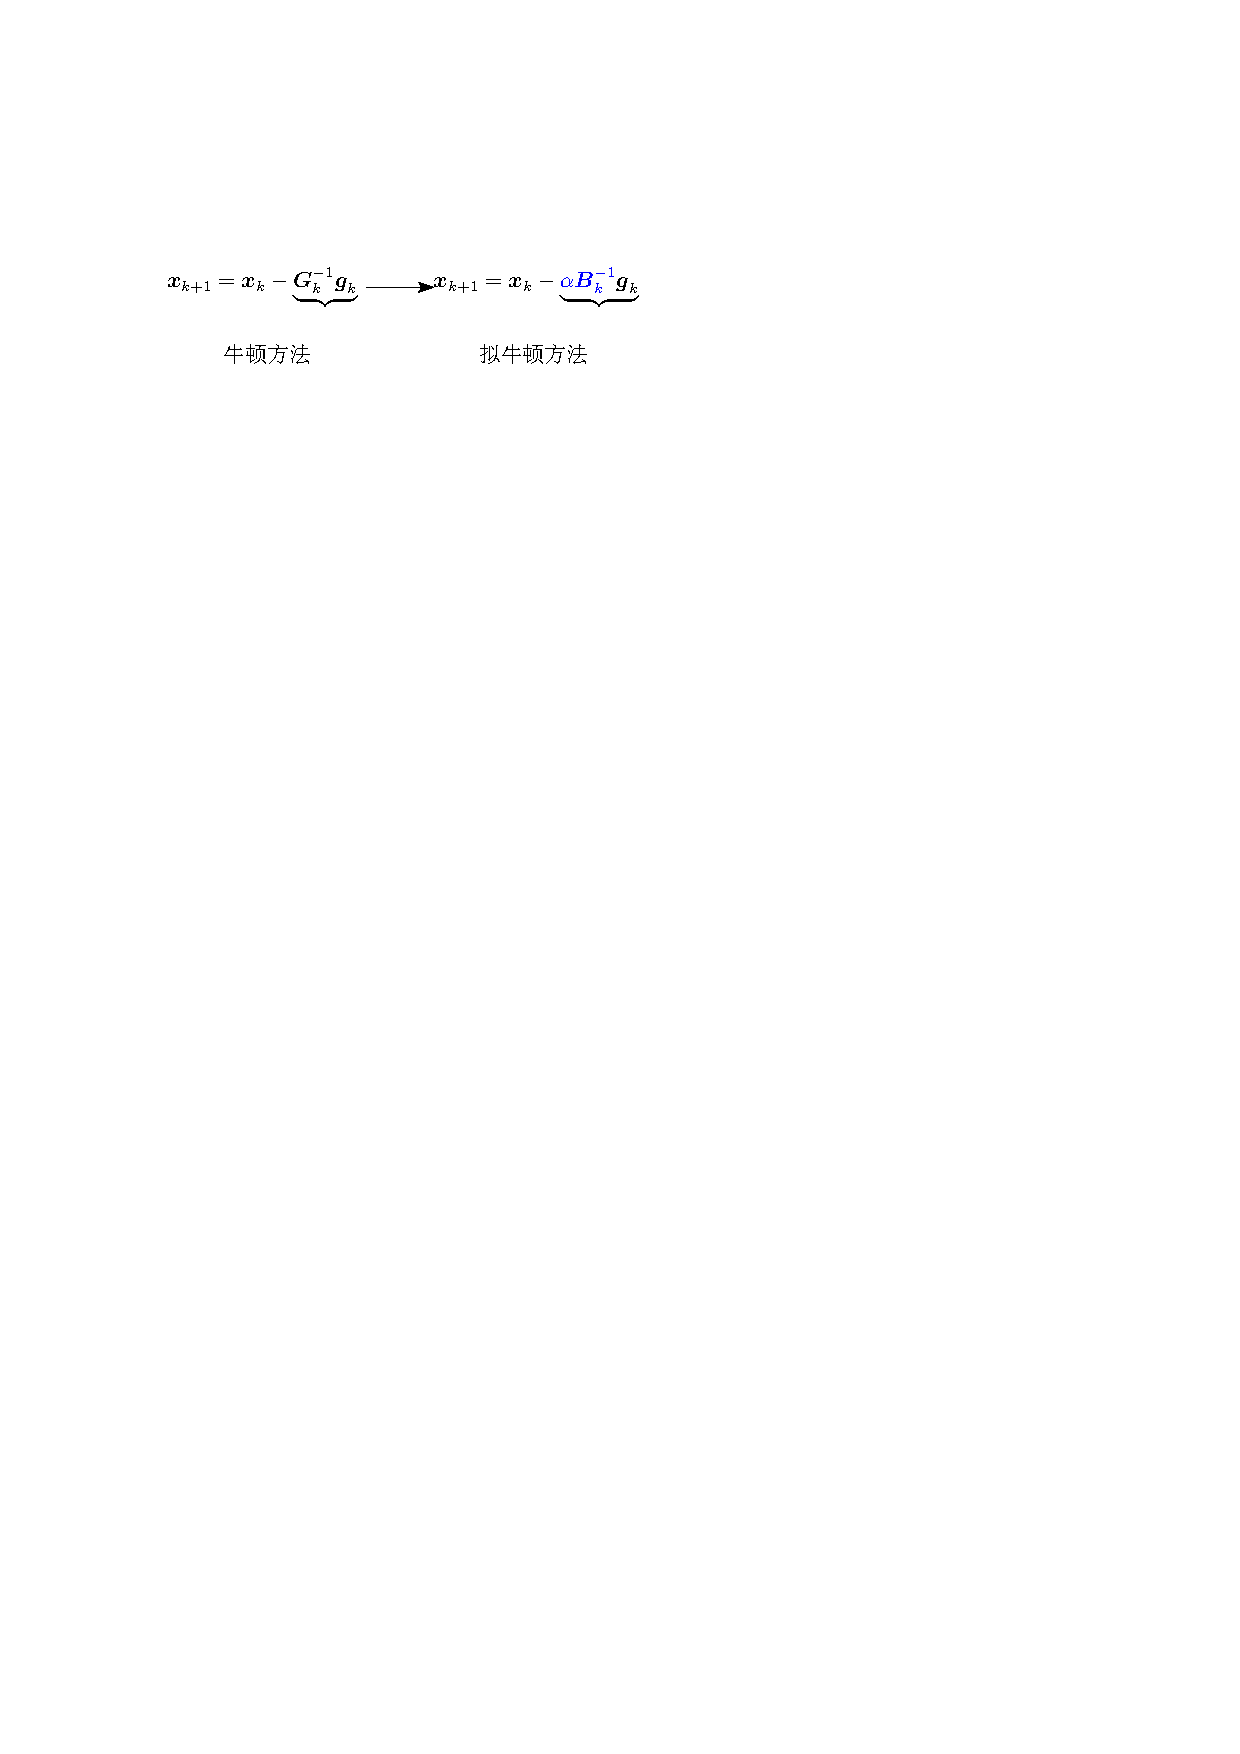
\includegraphics{image/拟牛顿方程.pdf}
    \end{figure}
\end{note}
考察目标函数梯度$\boldsymbol{g}(\boldsymbol{x})$在$\boldsymbol{x}_{k+1}$点的线性近似
\[
    \begin{array}{cl}
        & \boldsymbol{g}(\boldsymbol{x}_k)\approx \boldsymbol{g}_{k+1}+\boldsymbol{G}_{k+1}(\boldsymbol{x}_k-\boldsymbol{x}_{k+1})\\
        \implies   & \boldsymbol{g}_{k+1} - \boldsymbol{g}_{\boldsymbol{x}_k}\approx \boldsymbol{G}_{k+1}(\boldsymbol{x}_{k+1}-\boldsymbol{x}_k)\\
        \overset{\colorbox{blue!25}{$\begin{array}{l}
            \boldsymbol{y}_{k} = \boldsymbol{g}_{k+1}-\boldsymbol{g}_{k}\\
            \boldsymbol{s}_{k} = \boldsymbol{x}_{k+1}-\boldsymbol{x}_{k}
        \end{array}$}}{\implies} & \boldsymbol{y}_{k}\approx \boldsymbol{G}_{k+1}\boldsymbol{s}_{k}\\
        \overset{\boldsymbol{H}_{k+1} = \boldsymbol{B}_{k+1}^{-1}}{\implies} & \boldsymbol{H}_{k+1}\boldsymbol{y}_{k}\approx \boldsymbol{s}_{k}
    \end{array}
\]

得到重要结论
\[
    \textcolor{red}{\boldsymbol{H}_{k+1}\boldsymbol{y}_{k}\approx \boldsymbol{s}_{k}}
\]
\subsubsection{对称秩-1校正公式}
\begin{note}
    对称秩-1校正公式:
    \[
        \boldsymbol{H}_{k+1} = \boldsymbol{H}_{k} + \boldsymbol{v}_k\boldsymbol{v}_{k}^{\mathrm{T}}
    \]
    使用$\boldsymbol{H}_{k+1}\boldsymbol{y}_{k}\approx \boldsymbol{s}_{k}$两边同时乘以$\boldsymbol{y}_{k}$得到
    \[
        \boldsymbol{H}_{k}\boldsymbol{y}_{k} + \boldsymbol{v}_k\boldsymbol{v}_{k}^{\mathrm{T}}\boldsymbol{y}_{k} = \boldsymbol{s}_{k}
    \]
    得到
    \[
        \boldsymbol{v}_k = \dfrac{\boldsymbol{s}_{k}-\boldsymbol{H}_{k}\boldsymbol{y}_{k}}{\boldsymbol{v}_{k}^{\mathrm{T}}\boldsymbol{y}_{k}}
    \]
    所以对于$\boldsymbol{v}_k\boldsymbol{v}_{k}^{\mathrm{T}}$有
    \[
        \begin{array}{ll}
            \boldsymbol{v}_k\boldsymbol{v}_{k}^{\mathrm{T}} &= \dfrac{(\boldsymbol{s}_{k}-\boldsymbol{H}_{k}\boldsymbol{y}_{k})(\boldsymbol{s}_{k}-\boldsymbol{H}_{k}\boldsymbol{y}_{k})^\mathrm{T}}{(\boldsymbol{v}_{k}^{\mathrm{T}}\boldsymbol{y}_{k})(\boldsymbol{y}_{k}^{\mathrm{T}}\boldsymbol{v}_{k})}\\
            &=\dfrac{(\boldsymbol{s}_{k}-\boldsymbol{H}_{k}\boldsymbol{y}_{k})(\boldsymbol{s}_{k}-\boldsymbol{H}_{k}\boldsymbol{y}_{k})^\mathrm{T}}{\boldsymbol{y}_{k}^{\mathrm{T}}\boldsymbol{v}_{k}\boldsymbol{v}_{k}^{\mathrm{T}}\boldsymbol{y}_{k}}\\
            &=\dfrac{(\boldsymbol{s}_{k}-\boldsymbol{H}_{k}\boldsymbol{y}_{k})(\boldsymbol{s}_{k}-\boldsymbol{H}_{k}\boldsymbol{y}_{k})^\mathrm{T}}{(\boldsymbol{s}_{k}-\boldsymbol{H}_{k}\boldsymbol{y}_{k})^\mathrm{T}\boldsymbol{y}_{k}}
        \end{array}
    \]
    故而,
    \begin{equation}\label{eq:Rank-1_Hk+1}
        \boldsymbol{H}_{k+1} = \boldsymbol{H}_{k} + \dfrac{(\boldsymbol{s}_{k}-\boldsymbol{H}_{k}\boldsymbol{y}_{k})(\boldsymbol{s}_{k}-\boldsymbol{H}_{k}\boldsymbol{y}_{k})^\mathrm{T}}{(\boldsymbol{s}_{k}-\boldsymbol{H}_{k}\boldsymbol{y}_{k})^\mathrm{T}\boldsymbol{y}_{k}}
    \end{equation}
    \begin{enumerate}
        \item 取$\boldsymbol{x}_{0}\in\mathbb{R}^{n}$,矩阵$\boldsymbol{H}_{0}$(一般取$\boldsymbol{H}_{0} = \boldsymbol{I}$)和计算精度$\varepsilon$,令$k = 0$
        \item 计算搜索方向$\boldsymbol{d}_{k} = -\boldsymbol{H}_{k}\boldsymbol{g}_k$。令$\boldsymbol{x}_{k+1} = \boldsymbol{x}_{k}+\alpha_k\boldsymbol{d}_k$。其中, 步长由线搜索产生. 若$\|\boldsymbol{g}_{k+1}\|\leqslant \varepsilon$,算法停止;否则转下一步
        \item 利用
        \[
            \boldsymbol{H}_{k+1} = \boldsymbol{H}_{k} + \dfrac{(\boldsymbol{s}_{k}-\boldsymbol{H}_{k}\boldsymbol{y}_{k})(\boldsymbol{s}_{k}-\boldsymbol{H}_{k}\boldsymbol{y}_{k})^\mathrm{T}}{(\boldsymbol{s}_{k}-\boldsymbol{H}_{k}\boldsymbol{y}_{k})^\mathrm{T}\boldsymbol{y}_{k}}
        \]
        计算$\boldsymbol{H}_{k+1}$,令$k = k+1$,转步2
    \end{enumerate}
\end{note}
\subsubsection{DFP校正公式}
\begin{note}
    DFP校正公式:

    基于对称秩-1校正公式中的校正项
    \[
        \boldsymbol{H}_{k+1} = \boldsymbol{H}_{k} + \dfrac{(\textcolor{cyan!75}{\boldsymbol{s}_{k}}-\textcolor{blue!75}{\boldsymbol{H}_{k}\boldsymbol{y}_{k}})(\boldsymbol{s}_{k}-\boldsymbol{H}_{k}\boldsymbol{y}_{k})^\mathrm{T}}{(\boldsymbol{s}_{k}-\boldsymbol{H}_{k}\boldsymbol{y}_{k})^\mathrm{T}\boldsymbol{y}_{k}}
    \]
    对$\boldsymbol{H}_{k}$做如下对称秩-2校正
    \[
        \boldsymbol{H}_{k+1} = \boldsymbol{H}_{k} + a\textcolor{cyan!75}{\boldsymbol{s}_{k}\boldsymbol{s}_{k}^{\mathrm{T}}}+b\textcolor{blue!75}{\boldsymbol{H}_{k}\boldsymbol{y}_{k}\boldsymbol{y}_{k}^{\mathrm{T}}\boldsymbol{H}_{k}}
    \]
    利用$\textcolor{red}{\boldsymbol{H}_{k+1}\boldsymbol{y}_{k} = \boldsymbol{s}_{k}}$
    得到
    \[
        \cancel{\boldsymbol{H}_{k}\boldsymbol{y}_{k}} + a\textcolor{cyan!75}{\underline{\boldsymbol{s}_{k}}\boldsymbol{s}_{k}^{\mathrm{T}}}\boldsymbol{y}_{k}+\cancel{b\textcolor{blue!75}{\boldsymbol{H}_{k}\boldsymbol{y}_{k}\boldsymbol{y}_{k}^{\mathrm{T}}\boldsymbol{H}_{k}}\boldsymbol{y}_{k} } = \underline{\boldsymbol{s}_{k}}
    \]
    两边相等,故而
    \[
        a = \dfrac{1}{\boldsymbol{s}_{k}^{\mathrm{T}}\boldsymbol{y}_{k}},\quad b = -\dfrac{1}{\boldsymbol{y}_{k}^{\mathrm{T}}\boldsymbol{H}_{k}\boldsymbol{y}_{k}} 
    \]
    故而得到DFP校正公式
    \[
        \boldsymbol{H}_{k+1} = \boldsymbol{H}_{k} + \dfrac{\textcolor{cyan!75}{\boldsymbol{s}_{k}\boldsymbol{s}_{k}^{\mathrm{T}}}}{\boldsymbol{s}_{k}^{\mathrm{T}}\boldsymbol{y}_{k}} - \dfrac{\textcolor{blue!75}{\boldsymbol{H}_{k}\boldsymbol{y}_{k}\boldsymbol{y}_{k}^{\mathrm{T}}\boldsymbol{H}_{k}}}{\boldsymbol{y}_{k}^{\mathrm{T}}\boldsymbol{H}_{k}\boldsymbol{y}_{k}}
    \]
\end{note}


\begin{example}
    用DFP方法求解优化问题\Stars{5}{}
    \[
        \min f(\boldsymbol{x})=2x_{1}^{2}+x_{2}^{2}-4x_{1}+2
    \]
    解:容易计算$\boldsymbol{x}^* = (1,0)^{\mathrm{T}}$
    \[
        \nabla f(\boldsymbol{x}) = \begin{pmatrix}
            4x_1-4\\
            2x_2
        \end{pmatrix}
    \]
    \begin{enumerate}
        \item 取初始值$\boldsymbol{x}_0 = (2,1)^{\mathrm{T}}$,$\boldsymbol{H}_0 = \boldsymbol{I}$,则$\boldsymbol{g}_0 = (4,2)^{\mathrm{T}}$,沿着$\boldsymbol{d}_0 = -\boldsymbol{H}_0\boldsymbol{g}_0 = (-4,-2)^{\mathrm{T}}$精确线搜索得到$\alpha = \dfrac{5}{18}$
        
        新迭代点$\boldsymbol{x}_1 = \boldsymbol{x}_0+\alpha\boldsymbol{d}_0 = (\dfrac{8}{9},\dfrac{4}{9})^{\mathrm{T}}$
        进入下一次迭代
        \item 计算$\boldsymbol{x}_1 = \boldsymbol{x}_0+\alpha\boldsymbol{d}_0 = (\dfrac{8}{9},\dfrac{4}{9})^{\mathrm{T}}$,梯度$\boldsymbol{g}_0 = (-\dfrac{4}{9},\dfrac{8}{9})^{\mathrm{T}}$,进而计算
        \[
            \begin{aligned}
                \boldsymbol{s}_0&= \boldsymbol{x}_{1}-\boldsymbol{x}_{0} =\alpha_0\boldsymbol{d}_0=(-\frac{10}{9},-\frac{5}{9})^{\mathrm{T}}\\ 
                \boldsymbol{y}_0&=\boldsymbol{g}_1-\boldsymbol{g}_0=(-\frac{40}{9},-\frac{40}{9})^{\mathrm{T}}
            \end{aligned}
        \]
        得校正矩阵
        \[
            \boldsymbol{H}_1=\boldsymbol{H}_{0} + \dfrac{\textcolor{cyan!75}{\boldsymbol{s}_{0}\boldsymbol{s}_{0}^{\mathrm{T}}}}{\boldsymbol{s}_{0}^{\mathrm{T}}\boldsymbol{y}_{0}} - \dfrac{\textcolor{blue!75}{\boldsymbol{H}_{0}\boldsymbol{y}_{0}\boldsymbol{y}_{0}^{\mathrm{T}}\boldsymbol{H}_{0}}}{\boldsymbol{y}_{0}^{\mathrm{T}}\boldsymbol{H}_{0}\boldsymbol{y}_{0}}
            =\frac{1}{360}\begin{pmatrix}86&-38\\-38&305\end{pmatrix}
        \]
        沿着$\boldsymbol{d}_1=-\boldsymbol{H}_1\boldsymbol{g}_1=\dfrac{12}{51}(1,-4)^{\mathrm{T}}$精确线搜索得到$\alpha_1 = \dfrac{17}{36}$
        
        新迭代点$\boldsymbol{x}_{2}=\boldsymbol{x}_{1}+\alpha_{1}\boldsymbol{d}_{1}=\left(1,0\right)^{\mathrm{T}}=\boldsymbol{x}^{*}$,算法终止。
    \end{enumerate}
\end{example}

\subsection{信赖域方法}
优化模型$\min\limits_{\boldsymbol{x}\in\mathbb{R}^n}f(x)$

信赖域方法:$\boldsymbol{x}_{k+1}\gets \boldsymbol{x}_{k}$使得$f(\boldsymbol{x}_{k+1})<f(\boldsymbol{x})$

算法思想:构造目标函数的二阶近似,将其在当前点邻域内的最小值点作为新的迭代点。

构造$f(\boldsymbol{x}_k+\boldsymbol{d})$的二阶近似
\[
    m_{k}(\boldsymbol{d})=f(\boldsymbol{x}_{k})+\boldsymbol{g}_{k}^{\mathrm{T}}\boldsymbol{d}+\frac{1}{2}\boldsymbol{d}^{\mathrm{T}}\boldsymbol{B}_{k}\boldsymbol{d}
\]
其中$\boldsymbol{B}_{k}=\nabla^{2}f(\boldsymbol{x}_{k})$或者$\boldsymbol{B}_{k}\approx\nabla^{2}f(\boldsymbol{x}_{k}).$

\begin{note}
    信赖域子问题
    \[
        \min\{m_k(\boldsymbol{d})\mid\boldsymbol{d}\in\mathbb{R}^n,\lVert\boldsymbol{d}\rVert\leqslant\Delta_k\}.
    \]
    其中,$\Delta_{k}>0$为信赖域半径。

    设$\boldsymbol{d}_k$为其最优解。则目标函数与二次模型的近似度为
    \[
        f(\boldsymbol{x}_k+\boldsymbol{d}_k)-m_k(\boldsymbol{d}_k)=O(\|\boldsymbol{d}_k\|^2)
    \]
    若$\boldsymbol{B}_{k}=\nabla^{2}f(\boldsymbol{x}_{k})$,则
    \[
        f(\boldsymbol{x}_k+\boldsymbol{d}_k)-m_k(\boldsymbol{d}_k)=O(\|\boldsymbol{d}_k\|^2)
    \]
\end{note}
\begin{note}
    调整依据:$m_{k}(\boldsymbol{d}_k)$与$f(\boldsymbol{\boldsymbol{x}}_k+\boldsymbol{d}_k)$的近似度

    \begin{itemize}
        \item 预下降量:$\mathrm{Pred}_{k}=m_{k}(\boldsymbol{0})+m_{k}(\boldsymbol{d}_{k}),$
        \item 实下降量:$\mathrm{Ared}_k=f(\boldsymbol{x}_k)-f(\boldsymbol{x}_k+\boldsymbol{d}_k)$
        \item 下降比:$r_{k}={\dfrac{\mathrm{Ared}_{k}}{\mathrm{Pred}_{k}}}$
    \end{itemize}
\end{note}

\begin{note}
    信赖域算法:
    \begin{enumerate}
        \item 取$\hat{\Delta}>0,\boldsymbol{x}_{0}\in\mathbb{R}^{n},\Delta_{0}^{i}\in(0,\hat{\Delta}],\eta\in[0,\frac{1}{4}),\varepsilon\geqslant 0.$令$k = 0$
        \item 若$\|g_k\|\leqslant\varepsilon $,算法终止;否则进入下一步
        \item 解子问题$ \boldsymbol{d}_k=\arg\min\{m_k(\boldsymbol{d})\mid\boldsymbol{d}\in\mathbb{R}^n,\lVert\boldsymbol{d}\rVert\leqslant\Delta_k\} $
        
        计算$r_{k}={\dfrac{\mathrm{Ared}_{k}}{\mathrm{Pred}_{k}}}$

        若$r_{k}<\dfrac{1}{4}.$令$\Delta_{k+1}=\frac{1}{4}\Delta_{k}$;
        
        若$r_{k}>\dfrac34$,且$\|\boldsymbol{d}_{k}\|=\Delta_{k},$令$\Delta_{k+1}=\min\{2\Delta_{k},\hat{\Delta}\}$;

        否则,令$\Delta_{k+1} = \Delta_k$
        \item 若$r_{k}>\eta$,令$\boldsymbol{x}_{k+1} = \boldsymbol{x}_k+\boldsymbol{d}_k$
        
        否则,令$\boldsymbol{x}_{k+1}=\boldsymbol{x}_{k},k=k+1$,转2
    \end{enumerate}
\end{note}

\subsection{最小二乘问题}
最小二乘问题数学模型
\[
    \min\limits_{\boldsymbol{x}\in \mathbb{R}^n}\sum\limits_{i = 1}^{n}\left( y_i-\phi(\boldsymbol{x},t_i) \right)^2
\]
\begin{note}
    模型特点:
    \begin{itemize}
        \item $m\gg n$
        \item 目标函数为平方和形式,函数值非负
        \item 目标函数选取值恰当时,目标函数的最优值靠近零
    \end{itemize}
\end{note}
设$r_i(\boldsymbol{x}) = y_i-\phi(\boldsymbol{x},t_i)$模型可以写为
\[
    \min\limits_{\boldsymbol{x}\in \mathbb{R}^n}\boldsymbol{r}(\boldsymbol{x})^{\mathrm{T}}\boldsymbol{r}(\boldsymbol{x})
\]
其中$\boldsymbol{r}(\boldsymbol{x})=(r_1(\boldsymbol{x}),r_2(\boldsymbol{x}),\cdots,r_m(\boldsymbol{x}))^{\mathrm{T}}$。
\subsubsection{线性最小二乘}
数学模型
\[
    \min_{\boldsymbol{x}\in\mathbb{R}^n}\frac12\boldsymbol{r}(\boldsymbol{x})^{\mathrm{T}}\boldsymbol{r}(\boldsymbol{x})
\]
其中$\boldsymbol{r}(\boldsymbol{x})=\boldsymbol{Ax}-\boldsymbol{b},\boldsymbol{A}\in\mathbb{R}^{m\times n},\boldsymbol{b}\in\mathbb{R}^m$
问题转换为
\[
    \min_{\boldsymbol{x}\in\mathbb{R}^n}\frac12\|\boldsymbol{Ax}-\boldsymbol{b}\|^2
\]
\begin{theorem}
    线性最小二乘问题存在全局最优解。它有唯一最优解的充分必要条件是矩阵$\boldsymbol{A}$列满秩。
\end{theorem}
\subsubsection{非线性最小二乘}
数学模型
\[
    \min\limits_{\boldsymbol{x}\in \mathbb{R}^n} f(\boldsymbol{x}):=\frac12{\left\|\boldsymbol{r}(\boldsymbol{x})\right\|}^{2}
\]
\begin{note}
    梯度
    \[
        \nabla f(\boldsymbol{x})=\boldsymbol{g}(\boldsymbol{x})=\nabla\Bigl(\frac{1}{2}\boldsymbol{r}(\boldsymbol{x})^{\mathrm{T}}\boldsymbol{r}(\boldsymbol{x})\Bigr)=\boldsymbol{J}(\boldsymbol{x})^{\mathrm{T}}\boldsymbol{r}(\boldsymbol{x})=\sum_{i=1}^{m}r_{i}(\boldsymbol{x})\nabla r_{i}\bigl(\boldsymbol{x}\bigr)\colorbox{cyan!50}{数值乘以向量求和}
    \]
    其中
    \[
        \boldsymbol{J}(\boldsymbol{x})=D_x\boldsymbol{r}(\boldsymbol{x})=\begin{pmatrix}
            \frac{\partial r_1(\boldsymbol{x})}{\partial x_1}&\frac{\partial r_1(\boldsymbol{x})}{\partial x_2}&\cdots&\frac{\partial r_1(\boldsymbol{x})}{\partial x_n}\\
            \frac{\partial r_2(\boldsymbol{x})}{\partial x_1}&\frac{\partial r_2(\boldsymbol{x})}{\partial x_2}&\cdots&\frac{\partial r_2(\boldsymbol{x})}{\partial x_n}\\
            \vdots&\vdots&\ddots&\vdots\\
            \frac{\partial r_m(\boldsymbol{x})}{\partial x_1}&\frac{\partial r_m(\boldsymbol{x})}{\partial x_2}&\cdots&\frac{\partial r_m(\boldsymbol{x})}{\partial x_n}
        \end{pmatrix}
    \]
\end{note}
\begin{note}
    Hesse阵
    \[
        \begin{aligned}
            \nabla^{2}f(\boldsymbol{x})=\boldsymbol{G(x)}& =\sum_{i=1}^{m}\nabla r_{i}(\boldsymbol{x})\nabla^{\mathrm{T}}r_{i}(\boldsymbol{x})+\sum_{i=1}^{m}r_{i}(\boldsymbol{x})\nabla^{2}r_{i}(\boldsymbol{x})  \\
            & = \boldsymbol{J}(\boldsymbol{x})^{\mathrm{T}}\boldsymbol{J}(\boldsymbol{x})+\sum_{i=1}^{m}r_{i}(\boldsymbol{x})\nabla^{2}r_{i}(\boldsymbol{x}) \\
            &\overset{\triangle}{\operatorname*{=}}\boldsymbol{J}(\boldsymbol{x})^{\mathrm{T}}\boldsymbol{J}(\boldsymbol{x})+\boldsymbol{S}(\boldsymbol{x}).
        \end{aligned}
    \]
    其中
    \[
        \boldsymbol{S}(x)=\sum_{i=1}^{m}\boldsymbol{r}_{i}(\boldsymbol{x})\nabla^{2}\boldsymbol{r}_{i}(\boldsymbol{x})
    \]
\end{note}

\begin{note}
    牛顿算法
    \[
    \boldsymbol{x}_{k+1}=\boldsymbol{x}_k-\left(\boldsymbol{J}_k^\mathrm{T}\boldsymbol{J}_k+\boldsymbol{S}_k\right)^{-1}\boldsymbol{J}_k^\mathrm{T}\boldsymbol{r}(\boldsymbol{x}_k)
    \]
\end{note}
\begin{note}
    Gauss-Newton方法:
    当残量函数$\boldsymbol{r}(x)$很小时,$\boldsymbol{S}(\boldsymbol{x})=\sum_{i=1}^{m}r_{i}(\boldsymbol{x})\nabla^{2}r_{i}(\boldsymbol{x})$很小
    \[
        \boldsymbol{d}_{k}^{\mathrm{GN}}=-\bigl(\boldsymbol{J}_{k}^{\mathrm{T}}\boldsymbol{J}_{k}\bigr)^{-1}\boldsymbol{J}_{k}^{\mathrm{T}}\boldsymbol{r}(\boldsymbol{x}_{k})
    \]
    \[
        \boldsymbol{x}_{k+1} = \boldsymbol{x}_k+\alpha_k \boldsymbol{d}_{k}^{\mathrm{GN}} 
    \]
\end{note}